% Erros de modelo e de alcance, ordenados pela distância ao eixo da base (precisa de \usepackage{pgfplots})
% Feita para meia largura de página (dentro de uma minipage de 0,48\textwidth), sem \resizebox
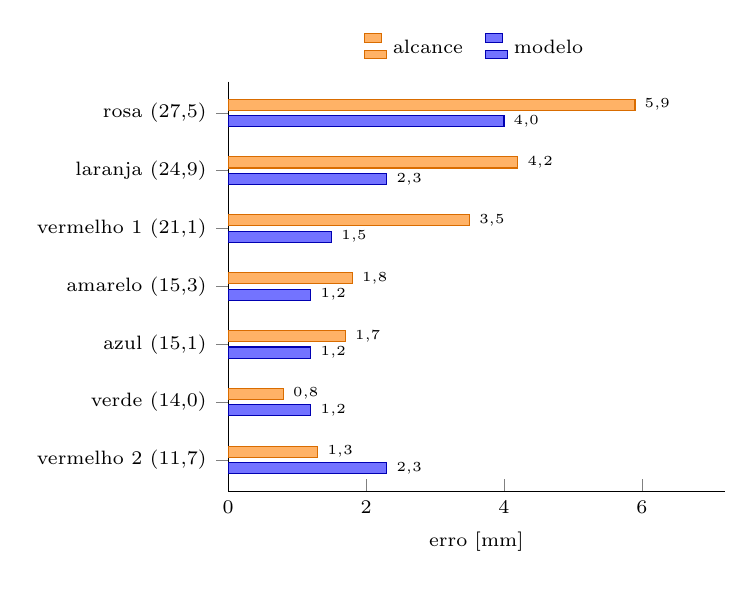
\begin{tikzpicture}
  \begin{axis}[xbar, bar width=4pt, scale only axis, width=0.52\linewidth, height=5.2cm,
      xmin=0, xmax=7.2, xlabel={erro [mm]},
      symbolic y coords={rosa, laranja, vermelho 1, amarelo, azul, verde, vermelho 2},
      ytick=data,
      yticklabels={{rosa (27,5)}, {laranja (24,9)}, {vermelho 1 (21,1)}, {amarelo (15,3)}, {azul (15,1)}, {verde (14,0)}, {vermelho 2 (11,7)}},
      y dir=reverse, enlarge y limits=0.09,
      tick label style={font=\scriptsize}, label style={font=\scriptsize},
      nodes near coords, every node near coord/.append style={font=\tiny},
      /pgf/number format/use comma, /pgf/number format/fixed, /pgf/number format/precision=1,
      /pgf/number format/fixed zerofill,
      legend style={at={(0.5,1.03)}, anchor=south, font=\scriptsize, draw=none, fill=none, legend columns=2, /tikz/every even column/.append style={column sep=6pt}},
      reverse legend,
      legend cell align=left,
      axis lines*=left, xtick={0,2,4,6}, xticklabels={0,2,4,6}]
    \addplot[fill=blue!55, draw=blue!70!black] coordinates
      {(4.0,rosa) (2.3,laranja) (1.5,vermelho 1) (1.2,amarelo) (1.2,azul) (1.2,verde) (2.3,vermelho 2)};
    \addplot[fill=orange!60, draw=orange!85!black] coordinates
      {(5.9,rosa) (4.2,laranja) (3.5,vermelho 1) (1.8,amarelo) (1.7,azul) (0.8,verde) (1.3,vermelho 2)};
    \legend{modelo, alcance}
  \end{axis}
\end{tikzpicture}